\documentclass[11pt]{article}
\usepackage[utf8]{inputenc}
\usepackage[T1]{fontenc}
\usepackage[margin=1in]{geometry}
\usepackage{amsmath,amssymb}
\usepackage{booktabs}
\usepackage{tabularx}
\usepackage{tikz}
\usetikzlibrary{arrows.meta,positioning,shapes.geometric}
\usepackage{graphicx}
\usepackage{hyperref}
\usepackage{enumitem}
\usepackage{listings}
\usepackage{xcolor}
\usepackage{caption}
\usepackage{setspace}
\usepackage{lmodern}
\usepackage{float}

\onehalfspacing

% Math and theorem environments (numbered by section)
\usepackage{amsmath, amssymb, amsthm}
\numberwithin{equation}{section}
\newtheorem{theorem}{Theorem}[section]
\newtheorem{lemma}[theorem]{Lemma}
\newtheorem{proposition}[theorem]{Proposition}
\newtheorem{definition}[theorem]{Definition}
\newtheorem{example}[theorem]{Example}
\hypersetup{
  colorlinks=true,
  linkcolor=blue!60!black,
  citecolor=blue!60!black,
  urlcolor=blue!60!black
}

\lstset{
  basicstyle=\ttfamily\small,
  keywordstyle=\color{blue!60!black},
  commentstyle=\color{green!40!black},
  stringstyle=\color{orange!70!black},
  showstringspaces=false,
  frame=single,
  breaklines=true,
  columns=fullflexible
}

% Author–year citations (JLC-friendly)
% \usepackage[round,authoryear]{natbib}
\usepackage[numbers,sort&compress]{natbib}
% \bibliographystyle{plainnat}

% Simple anonymization toggle (no structural impact)
\newif\ifjlcAnon
\jlcAnonfalse           % set to \jlcAnonfalse for camera-ready


\title{Epistemic State Updates in LLM Agents via Public Announcement and Graded Modal Logic}
% to anonymize without changing section structure.
\ifjlcAnon
  % For submission:
  \author{Anonymous Submission}
  \date{}
\else
  % For camera-ready (fill in later):
  \author{Justin Mullins\thanks{Johns Hopkins University, Whiting School of Engineering} \and John Symons\thanks{University of Kansas, Center for Cyber Social Dynamics}}
  \date{\today}
\fi

\begin{document}

\maketitle

\begin{abstract}
Large Language Model (LLM) agents reason and act in dynamic environments but often lack an explicit account of what they know or believe at each step. This paper introduces a lightweight epistemic state management framework grounded in Public Announcement Logic (PAL) and graded modal logic. We treat observations, tool results, and internal inferences as \emph{announcements} that transform an agent’s knowledge state. Each announcement updates a minimal log $\Sigma$ that serves as a filter on the agent’s possible worlds, maintaining consistency while avoiding full model enumeration. We extend PAL with graded belief operators to represent uncertainty and show how these can model belief revision and bounded rationality. Our framework enables explicit, inspectable reasoning in LLM agents, improving self-consistency, interpretability, and epistemic awareness. We conclude with implementation sketches and evaluation plans for benchmarking epistemic reasoning in LLM agents.
\end{abstract}

\noindent\textbf{Keywords:} dynamic epistemic logic, public announcement logic, graded belief, belief revision, LLM agents, epistemic reasoning

% ===============================================================================================

% Auto-generated from DOCX
\section{Introduction}
Large Language Models (LLMs) have rapidly become central components in AI agents, powering complex decision-making and interactive workflows. However, a persistent challenge is how an LLM-based agent represents and updates its knowledge and beliefs about the world as it interacts. Current LLM agents often rely on implicit state in the prompt (e.g. chat history or scratchpad) and learned language patterns rather than an explicit, verifiable model of what the agent knows or believes at each step. This can lead to inconsistencies, hallucinations, or failures to recognize what information is missing. Recent evaluations of epistemic agency in LLMs, understood as the capacity to construct, adapt, and monitor beliefs, indicate that while modern LLMs show rudimentary abilities, they still have significant limitations in flexible belief updating and self-consistency\cite{reflection-bench}. In particular, advanced models struggle with higher-order reasoning and meta-reflection, i.e. reflecting on their own knowledge and correcting it when faced with new evidence\cite{reflection-bench}. These limitations motivate a more principled approach to managing an agent's state of knowledge in dynamic environments.

In this paper, we propose a practical, theoretically grounded framework for enabling belief and knowledge updates in LLM-based agents by drawing on epistemic logic, the logic of knowledge and belief, and its dynamic extension, Public Announcement Logic (PAL). Epistemic logic provides a rigorous way to describe an agent's knowledge in terms of possible worlds or states of affairs, and PAL describes how knowledge changes when new information is announced. The key idea is to treat events in an LLM agent's workflow (observations, tool outputs, intermediate conclusions, etc.) as analogous to announcements that update the agent's knowledge state. By formalizing these updates, we can maintain an explicit minimal representation of the agent's state, for example a log of facts learned or a summary of the current state, without needing to enumerate all possible world states or propositions. Each new piece of information eliminates incompatible possibilities from consideration, focusing the agent's belief state. Intuitively, to say an agent knows a fact means that fact holds in all situations the agent considers possible\cite{del-sep}. Conversely, acquiring new information that is certain and true can be seen as ruling out all previously possible situations where that information would be false\cite{del-sep}. Public announcements capture this process: a truthful announcement of a proposition $F$ causes all non-$F$ worlds to be discarded from every agent's set of epistemic possibilities\cite{del-sep}. Our framework brings this model-change semantics into LLM agents in a lightweight way by recording and enforcing the constraints introduced by each announcement (new information) rather than storing an explicit list of all possible worlds.

We emphasize minimality and practicality in the proposed approach. Rather than constructing full Kripke models with millions of possible worlds for an LLM's rich knowledge space, we maintain only the essential state updates, such as a list of facts confirmed or assumptions made, that serve as epistemic filters on the space of possibilities. For instance, if the agent receives a tool result confirming a fact, that fact is added to a knowledge base (or context window for the LLM), and any future reasoning implicitly treats worlds violating that fact as impossible. This is analogous to how in state estimation, obtaining one observation can exclude ``the vast majority of the universe'' of prior possibilities\cite{espf}, imposing ``hard bounds on the set of plausible states''\cite{espf}. The agent's knowledge state thus becomes a progressively narrower admissible region of possibilities consistent with everything it has observed or deduced so far, much like an epistemic support filter contracts a region of plausible states in response to new evidence\cite{espf}. Crucially, we do not require the agent to enumerate or generate all the eliminated possibilities explicitly; we only store the log of announcements (facts, observations, etc.) that have been accepted. This log or state summary implicitly defines the set of possible worlds remaining (those in which all logged facts are true). In effect, the agent's knowledge base is the conjunction of all announcements it has received, serving as a consistent, minimal record of its current knowledge. As long as this record is kept manageable in size (through techniques like summarization or forgetting of irrelevant details), the approach scales without the combinatorial explosion of explicitly tracking every hypothetical state.

The contributions of this work are as follows. First, we provide a self-contained overview of key concepts from epistemic logic and PAL that are relevant to AI agent design, including possible worlds semantics, knowledge vs. belief modalities, and public announcement updates, illustrated with concrete examples. We extend this with discussion of graded or fuzzy modal logics, which allow reasoning about degrees of belief or uncertainty, an important consideration for real-world LLM agents that operate under uncertainty and are not logically omniscient. Second, we propose a framework for an ``epistemic state management layer'' in an LLM agent architecture. This layer treats the agent's internal chain-of-thought and interactions as a sequence of epistemic actions (public announcements being the simplest) that update a compact state representation (like a knowledge log or set of constraints). We describe how this can guide the agent's action selection and reasoning: for example, the agent can query its knowledge state to decide if a certain fact is known or if further information-gathering is needed (akin to planning with knowledge preconditions\cite{Bolander2017Gentle}). We give implementation examples showing how tool calls and observations translate into public announcements that update the agent's state, and how minimal data structures (e.g. sets of propositions, or simple epistemic graphs) can simulate richer epistemic models. Third, we discuss how the framework can be implemented in practice without generating or storing all possible propositions an LLM might handle. We highlight techniques like representing knowledge states by formulas or constraints rather than explicit world lists, and using the LLM's own reasoning capability to infer consequences on the fly rather than precomputing all logical entailments. The agent is therefore resource-bounded and non-omniscient by design, acknowledging the practical limits on memory and computation. This stance aligns with real-world deployment and ``bounded rationality'' considerations\cite{pal-predictive}.

Finally, we position this work as a step toward structured cognition in LLM systems. By structured cognition, we mean an architecture where the flow of thought and action is modulated by an internal model of what is known, unknown, or conjectured, much like human reasoning keeps track of beliefs and uncertainties. Our epistemic update protocol can serve as a generic layer that could be added to various LLM agent frameworks (from conversational assistants to autonomous tool-using systems) to enhance consistency and reliability. We draw parallels to classical agent models like the belief-desire-intention (BDI) architecture, which explicitly maintains a set of beliefs (informational state) separate from goals and plans. In fact, the term belief is used (rather than ``knowledge'') in BDI to allow for the possibility that the agent's information might be wrong. Our framework similarly accounts for uncertainty and error: not every piece of information an LLM uses needs to be absolutely true, because some announcements might represent the agent's beliefs with some degree of confidence. We discuss how graded modal logic or probabilistic updating (as studied in dynamic epistemic logic extensions) can be incorporated to handle such cases. The overarching vision is that LLM agents can benefit from a logic-informed cognitive layer that ensures their evolving knowledge remains as consistent, minimal, and task-relevant as possible, even as they operate under partial observability and uncertainty.

The remainder of this paper is organized as follows. Section 2 (Background) reviews core concepts in epistemic logic, public announcement logic, and graded modal logics, grounding the discussion with simple examples and references to prior work in AI that combines logic and planning. Section 3 (Framework Design) presents our proposed approach to modeling LLM agent knowledge states and updates, including data structures for minimal epistemic state representation and algorithms for update and query. We illustrate the framework with an example workflow of an LLM agent interacting with a tool and updating its beliefs. Section 4 (Implementation Considerations) addresses practical issues such as partial observability, handling uncertainty (via fuzzy or probabilistic modalities), ensuring scalability through bounded reasoning and summarization, and integrating the logic-based state mechanism with the LLM's prompt or memory. Section 5 (Discussion) explores the implications of this approach, comparing it to related approaches (like chain-of-thought prompting and neuro-symbolic methods), and highlighting open challenges such as the limits of LLM introspection, potential inconsistencies, and how to evaluate epistemic reasoning in LLM agents. We suggest some directions for empirical evaluation, including adapting existing theory-of-mind or knowledge reasoning benchmarks to test LLM agents with and without epistemic update mechanisms. Finally, Section 6 (Conclusion) summarizes our findings and contributions. As a playful aside, we also propose a tentative name for this epistemically-informed agent framework, inspired by the rich tradition of logic and epistemology, to capture the spirit of the approach.


% Auto-generated from DOCX
\section{Background: Epistemic Logic and Public Announcements}
\subsection{Knowledge, Belief, and Possible Worlds}
Epistemic logic is the branch of modal logic that formalizes reasoning about knowledge and belief. In epistemic logic, one typically introduces a modal operator $K_i$ to mean ``agent $i$ knows that...'', and similarly $B_i$ for ``agent $i$ believes that...'', in the context of multi-agent systems\cite{vanBenthem2011LogicalDynamics}. The semantics of these operators is often given by Kripke models (possible worlds models). A Kripke model for epistemic logic consists of a set of possible worlds (states of affairs), and for each agent $i$, an accessibility relation $R_i$ between worlds that encodes which worlds agent $i$ considers possible from a given world\cite{del-sep}. Intuitively, if the actual world is $w$, the set of worlds ${v \mid w R_i v}$ represents the epistemic alternatives that agent $i$ cannot distinguish from the actual world. Then $K_i \varphi$ (agent $i$ knows $\varphi$) is true at world $w$ if and only if $\varphi$ is true in all worlds $v$ accessible via $R_i$ from $w$\cite{del-sep}. In plainer terms: an agent knows $\varphi$ exactly when, given everything the agent has observed or been told, $\varphi$ holds in every situation the agent regards as possible. For example, if $\varphi$ means ``the key is in the drawer'' and the agent knows this, then any world the agent thinks might be the real one must have the key in the drawer; if there were even one conceivable world (consistent with the agent's information) where the key is elsewhere, the agent would not truly know $\varphi$.

The possible-worlds semantics elegantly captures the information content of knowledge. Knowledge rules out possibilities. As the agent gains more information, it rules out more worlds from consideration, thereby narrowing down the set of candidates for reality. Conversely, if an agent is uncertain about something, it means multiple possible worlds (differing on that fact) are still in its epistemic range. Knowledge in the standard modal logic treatment is usually assumed to be veridical (if $K_i \varphi$ then $\varphi$ is true) and agents are logically omniscient (they know all logical consequences of their knowledge). These assumptions correspond to properties of the accessibility relation like reflexivity, transitivity, and Euclideanness (characterizing the modal system S5 for knowledge)\cite{del-sep}. In practice, logical omniscience is an unrealistic idealization. Real agents (and LLMs) have bounded reasoning capabilities and may not instantly deduce all implications of what they know\cite{pal-predictive}. We will later relax these assumptions when mapping epistemic logic to practical LLM agents. The distinction between knowledge and belief is also important. Doxastic logic uses a modality $B_i$ for belief, which does not require truth (an agent can believe $\varphi$ even if $\varphi$ is false) and often corresponds to a weaker modal system (e.g. KD45 instead of S5). In AI agent architectures like BDI, a belief base represents the agent's informational state, acknowledging that some beliefs could be wrong or revised later. In our framework, we allow the LLM agent's state to include beliefs that might be probabilistic or defeasible, not just certainties, which provides a bridge to the graded logic discussion that follows.

To make these ideas concrete, consider a simple scenario: an agent trying to locate an object in one of two boxes. Initially, the agent doesn't know which box contains the object. This ignorance can be modeled by two possible worlds: $w_1$ (object in Box A) and $w_2$ (object in Box B), and the agent considers both $w_1$ and $w_2$ possible. Thus the agent does not know the object's location, because in one possible world the proposition ``object is in A'' is true, and in another it's false. Now suppose the agent looks into Box A and finds it empty. This observation eliminates all worlds where the object was in A (namely $w_1$) from the agent's epistemic alternatives. Now only $w_2$ remains possible, in which the object must be in B. At that moment, the agent knows the object is in Box B. We didn't need to explicitly list out every hypothetical scenario. It was enough to capture that the agent's prior knowledge allowed two possibilities, and after the observation only one. This example reflects how observations function as epistemic updates, ruling out possibilities and thereby converting uncertainty into knowledge. It is analogous to a logical inference as well: from ``Box A is observed empty'' the agent can infer ``object is in B'' given the prior that it's in A or B. The power of epistemic logic is in providing general tools to analyze such reasoning patterns, especially in multi-step or multi-agent settings where agents may reason about each other's knowledge (though in this paper we mostly focus on a single agent and the environment).

\subsection{Public Announcement Logic (PAL) and Knowledge Updates}
Public Announcement Logic (PAL) is a framework within dynamic epistemic logic that explicitly considers how knowledge changes when a truthful announcement is made publicly to all agents\cite{vanDitmarsch2007DEL,Baltag1998PAL}. The classic PAL operator is of the form $[!\psi]$ which, when prefixed to a formula $F$, means ``after a public announcement of $\psi$, $F$ holds.'' An announcement is assumed to be a truthful, transparently heard statement that all agents receive (and believe). The effect of an announcement $\psi$ in a Kripke model is to eliminate any possible world where $\psi$ is false\cite{del-sep}, because once $\psi$ is announced, all agents know $\psi$ is true (and know that others know, etc., though we won't delve deeply into common knowledge here). In the updated model, the set of worlds is shrunk to $W':={ w \in W \mid w \models \psi }$, and the accessibility relations are restricted accordingly. Thus, PAL provides a formal account of information-driven model transformations.

For example, consider the well-known Muddy Children Puzzle often cited in PAL contexts\cite{del-sep}: a group of children might each have mud on their forehead or not, and they can see others but not themselves. An announcement like ``At least one of you has muddy forehead'' (which they all hear) can, through its successive implications, lead them to deduce who is muddy after a few rounds of reasoning. PAL neatly models each announcement and its effect on the group's knowledge. For a simpler illustration, let's revisit the one-agent box scenario above in PAL terms. Initially, the agent doesn't know the object's location ($
\neg K(\text{in A})$ and $
\neg K(\text{in B})$ both hold). Now, the agent looking into Box A and seeing it empty can be treated as the environment making an announcement to the agent: ``Box A is empty.'' This announcement is effectively public to the agent's mind (though there is only one agent, ``public'' means the agent fully trusts the observation). Applying the PAL semantics, the agent's epistemic model is updated by dropping any world where ``Box A is empty'' is false, i.e., any world where the object was in A. The result is that in the updated model the agent knows ``object is in B.'' Formally, if $\psi$ is ``Box A is empty'' and $F$ is ``I know the object is in B,'' PAL would allow us to conclude $[!\psi] K(\text{in B})$. This is a rather trivial case, but it shows the mechanics: announcements reduce uncertainty by filtration.

One important aspect of PAL is that announcements can be about any proposition, including those describing agents' knowledge. This allows modeling higher-order knowledge updates (e.g. ``Announcing $\psi$'' might let agent 1 know that agent 2 now knows $\psi$, etc.). In our context of LLM agents, we mostly consider announcements of factual information from the environment or results of the agent's own actions. These are akin to sensing actions in AI planning, steps that reveal information about the world. Indeed, epistemic planning research often uses dynamic epistemic logic to model how an agent can perform actions that change not the physical world but the agent's knowledge state\cite{Bolander2017Gentle}. For instance, an epistemic planning problem might include an action ``inspect Box A'' that has the conditional effect of telling the agent whether Box A is empty or not. Such an action corresponds to a public announcement (to the agent itself) of the observation's outcome. Bolander (2017) notes that dynamic epistemic logic provides a natural and expressive way to formalize these scenarios, avoiding the need to hard-code knowledge changes in the logic of actions\cite{pal-survey}. Instead, the knowledge change falls out from the semantics of announcement: after the action, the agent's possible worlds are automatically restricted to those consistent with the observation.

In summary, PAL gives us a way to reason about belief state transformations due to new information. For a large language model agent, we can treat many events as announcements: - A tool API call result that returns some data can be an announcement of that data's value. - A user instruction or answer revealed is an announcement from the environment's perspective. - The agent's own conclusions or reflections could even be treated as (private) announcements to itself, solidifying a new piece of derived knowledge.

PAL assumes announcements are truthful and believed. In real settings, what if an agent receives misinformation or an observation that could be noisy? The standard PAL model would lead the agent to believe a falsehood, which might later need revision. Handling such cases leads into belief revision or more complex dynamic logics (e.g. plausibility models and action plausibility updates\cite{del-sep}). For now, we note that our framework can incorporate belief updates that are not certain truths by using a graded approach (discussed later). But the simplest case, which we focus on first, is where the agent treats incoming info as reliable (at least until evidence suggests otherwise).

\subsection{Graded and Fuzzy Modal Logics for Uncertainty}
Classical epistemic logic and PAL operate mostly in black-and-white terms: either a proposition is considered possible or it is eliminated; either something is known or it isn't. However, practical AI agents often deal with degrees of belief or uncertainty. A large language model might have a probability or confidence distribution over possible answers, or might consider some facts more plausible than others given its prior knowledge. To capture this within a logical framework, researchers have developed graded modal logics and fuzzy logic extensions of epistemic logic. The basic idea is to allow statements like ``agent $i$ believes $\varphi$ with at least degree $0.8$'' or ``with probability at least $0.8$.'' A graded modal operator might be written $B_i^{\ge k} \varphi$ meaning ``agent $i$ believes $\varphi$ with degree at least $k$'' on some scale. In other approaches, one can attach a numerical plausibility or probability to each possible world, instead of a binary possible/impossible classification\cite{del-sep}.

One influential framework is the use of plausibility models in dynamic epistemic logic for belief\cite{del-sep}. In a plausibility model, each agent's uncertainty is represented by a ranking or partial order over worlds (rather than just an accessibility set)\cite{del-sep}. For example, an agent might consider many worlds possible, but some are deemed more plausible than others. A belief could then be defined as truth in all the most plausible worlds (typically formalized via a ``selection function'' or spheres of plausibility around the actual world, following Grove's system of spheres analogy\cite{del-sep}). When new information arrives that is uncertain. For example, the agent may encounter situations where the event is not a guaranteed truthful announcement but an observation with some chance of error, the agent can update plausibilities rather than completely eliminate worlds. If the agent is told ``$\psi$ is likely true,'' it might boost the plausibility of worlds where $\psi$ holds, without entirely discarding $
eg\psi$ worlds.

Another approach is probabilistic epistemic logic, which assigns probabilities to sets of worlds and allows formulas like ``agent $i$ assigns at least 80\% probability to $\varphi$.'' Dynamic epistemic logics have been extended with Bayesian update operators to model agents performing Bayesian belief updates on their probability distributions when events occur\cite{del-sep}. For instance, after observing some evidence, an agent might update the probabilities of various possibilities according to Bayes' rule. This is analogous to a ``soft'' announcement which reduces probability of some worlds to zero (if the evidence has zero probability in them) and reweights others proportionally.

In the context of LLM agents, why do graded or fuzzy modalities matter? Because LLMs do not intrinsically operate with a clear true/false world model. Instead, an LLM has an internal representation (in its weights and activations) that can be seen as encoding likelihoods or confidence about various statements. When an LLM ``considers'' a question, it often produces probabilities for different answers. We could interpret an LLM's 90\% confidence in an answer as the agent believing that answer with degree 0.9. If the agent then finds conflicting evidence, it might lower that confidence. Representing these changes in a logical way could involve saying ``Belief(p) dropped from 0.9 to 0.1 after observing X.'' While our framework in this paper primarily treats the knowledge state in a symbolic fashion (for clarity of exposition), it can be generalized to allow weighted beliefs. For example, we might maintain not just a set of known facts, but a set of believed propositions with confidence scores. Updates would then use rules akin to Dempster-Shafer evidence combination or Bayesian updates rather than simple set subtraction.

There are formalisms specifically for fuzzy modal logic that allow truth values in $[0,1]$. For instance, Li and Gong (2022) present a graded many-valued modal logic G(S5) with definitions of graded truth and rough truth degrees for modal formulas\cite{graded-many-valued}. Such formalisms could be applied to model an LLM agent's partial knowledge. Imagine the agent has a fuzzy belief like ``I suspect with 0.7 confidence that the user is asking about sports.'' This might be represented in a graded epistemic logic and updated as the conversation continues.

For practical implementation, one need not fully formalize a probability distribution. A simpler method used in some agent systems is to keep multiple possible hypotheses around. For instance, an agent might have a shortlist of plausible worlds or scenarios it's considering, rather than one fixed believed world. This connects to the idea of hypothetical or counterfactual reasoning; the agent might say ``If hypothesis H were true, I'd expect observation O; since I observed not-O, H becomes less plausible.'' Some LLM-based reasoning frameworks attempt to do this implicitly by prompting the model to consider alternatives (``let's assume X, see if it leads to contradiction''). Our logic-based approach could make it more systematic: the state could be a set of possibilities with labels like ``eliminated'' or ``active'' and perhaps a score. A graded announcement could then downgrade the plausibility of worlds failing the announcement without fully deleting them, reflecting uncertainty.

In summary, graded epistemic logics provide the tools to represent uncertainty and belief strength, which are crucial for realistic agent reasoning under partial information. In this paper, we will mostly illustrate using the simpler crisp announcements (which either completely rule things out or not) for clarity. But it should be kept in mind that this can be generalized. The framework we propose can function in a ``belief mode'' where announcements act like Bayesian evidence: rather than an all-or-nothing elimination, an update could mark some knowledge as uncertain or likely. For instance, if an LLM agent reads a single article claiming something controversial, it might not fully ``know'' that claim as true, but it might assign it a belief status pending further verification. Implementing this might mean the agent's knowledge log records the claim with a note ``unverified'' or a confidence level, and the decision-making layer treats it accordingly (e.g. it might seek a second source to confirm, rather than acting on it blindly).

\subsection{LLM Agents and Existing Approaches to State Management}
Before diving into our framework, it is useful to review how current LLM-based agent systems handle state and memory, and where the gaps are. Traditional AI planning systems had explicit world models and belief states, but many modern LLM agents use a mostly implicit approach:
\begin{itemize}
  \item \textbf{Prompt history as memory.} The conversation or action history is kept as text and provided to the LLM in each prompt (possibly truncated or summarized if it grows too long). This gives the model context but leaves the information unstructured, so the LLM must infer which statements are still valid.
  \item \textbf{Tool-assisted reasoning transcripts.} Frameworks such as ReAct interleave thoughts and tool calls, storing them in a transcript that acts as a log of what the agent has done and learned. Because the transcript lacks enforced logical constraints, consistency depends entirely on the LLM's learned behavior.
  \item \textbf{Long-term memory modules.} Cognitive architectures like Generative Agents maintain evolving memory streams with summarization and retrieval components\cite{generative-agents}. They store events rather than a full world state, which aligns with our minimal representation, yet they still rely on prompting the LLM to infer the implications of new observations. Our framework can provide the formal backbone that automatically records consequences such as marking $X$ as completed when an observation says ``X is now done.''
  \item \textbf{Symbolic augmentations.} Other work combines LLMs with knowledge graphs or symbolic modules so that facts can be stored and queried more reliably than in the model's parameters. These systems demonstrate the value of a factual database; we generalize this idea by maintaining the ``database of known facts'' under announcement-style update rules, including meta-facts about unknowns or assumptions.
\end{itemize}

These patterns show that current systems rely on memory mechanisms without a formally specified update semantics.

In the planning and multi-agent systems community, epistemic planning has tackled the problem of agents planning under uncertainty and with information-producing actions\cite{pal-survey,dynamic-term-modal}. Techniques include compiling epistemic logic into classical planning via state enumeration or using satisfiability solvers on epistemic formulas. However, these techniques often struggle with scale because the space of possible knowledge states can blow up combinatorially (especially with nested beliefs about other agents). LLM agents differ in that we have a powerful pattern-matching and generative core (the LLM) that can do a lot of the heavy lifting if guided properly, rather than having to explicitly enumerate states. This suggests a hybrid approach: use logic to maintain a coarse but sound state representation (prevent obvious contradictions, know what needs to be known, etc.), and use the LLM for the ``heavy'' reasoning and language generation conditioned on that state.

To underscore the need for explicit state tracking, consider an example from a dialog or interactive fiction setting. Without an explicit state, an LLM may forget a fact stated only a while ago, or it may inadvertently introduce inconsistencies (like mentioning an object that was taken earlier as if it's still present). Humans maintain an internal model of the conversation's common ground, a form of common knowledge, to avoid such mistakes. Our framework effectively gives the LLM a pseudo-common-ground model: the log of announcements can be thought of as maintaining common knowledge between the agent and itself (and the user, if applicable) of what has been said or observed. PAL includes common knowledge, formalized as the greatest fixpoint of iterated ‘everyone knows’ ($E^*$) over a group. For a single agent, under positive introspection (axiom 4), common knowledge of $\varphi$ is equivalent to $K\varphi$; without 4 it is stronger than a single $K\varphi$.

In conclusion, existing LLM agent methodologies implicitly recognize the importance of remembering and updating state (through logs, memories, context windows, etc.), but they often lack a formal semantics for those updates. This can lead to either oversights (the agent doesn't realize what it should logically infer) or hallucinations (the agent asserts something inconsistent because it failed to notice a contradiction). By importing the principles of epistemic logic and PAL, we aim to provide a clear semantics for the agent's memory and a protocol for updating it that ensures logical consistency in a minimal, tractable way.


% Auto-generated from DOCX
\section{Framework Design: Epistemic Workflows for LLM Agents}
In this section, we present the design of our epistemic state management framework for LLM-based agents. The framework can be viewed as a protocol layer that operates between the agent's cognition (LLM-driven reasoning and language generation) and its environment interactions. This layer maintains a representation of the agent's knowledge/belief state and provides two primary operations:
\begin{enumerate}
  \item \texttt{update(state, announcement)}: Incorporate a new piece of information (announcement) into the agent's state, modifying the state (usually by adding a constraint or fact) and possibly triggering internal consequences.
  \item \texttt{query(state, formula)}: Allow the agent or an external evaluator to inspect what is known or believed in the current state (e.g. check if a certain proposition is entailed by the knowledge log).
\end{enumerate}

We first describe the choice of knowledge representation, then the update mechanism (inspired by PAL), and then how this ties into the agent's decision-making (action selection and planning). An illustrative example is provided to tie everything together.

\subsection{Minimal State Representation as Epistemic Filter}
The agent's epistemic state $\Sigma$ at any time is represented in a minimal, declarative form. We can think of $\Sigma$ as essentially a list (conjunction) of formulas that the agent currently takes to be true (announcements it has received or assumed). Initially, $\Sigma$ may contain the agent's prior knowledge or assumptions about the world. For instance, if the agent starts a task knowing some background facts, those would be in $\Sigma_0$. If the agent has no specific knowledge apart from logical axioms, $\Sigma_0$ might be just tautologies or even empty (meaning all worlds are possible initially).

As the agent proceeds, $\Sigma$ is updated. There are design choices for how to implement $\Sigma$:
\begin{itemize}
  \item \textbf{Explicit list of propositions.} Treat $\Sigma$ as $\{\varphi_1, \varphi_2, \ldots, \varphi_n\}$, ensuring the set remains consistent when new announcements arrive. Inconsistencies can be handled by rejecting or revising facts.
  \item \textbf{Single conjunctive formula.} Maintain $\Sigma$ as the conjunction of all known facts, which is useful when interfacing with solvers or prompting the LLM with a compact summary.
  \item \textbf{Structured state.} Encode $\Sigma$ as a graph or database when the domain has rich structure. For many LLM tasks, however, an unstructured fact list is sufficient.
\end{itemize}

We opt for a simple model: treat $\Sigma$ as a set of facts the agent believes to be true. Initially, $\Sigma_0$ might be empty or contain basic context. For example, if the agent is solving a puzzle, $\Sigma_0$ could list the puzzle's givens. If multiple agents were involved, each would have their own $\Sigma_i$, but here we focus on one agent.

Now, how does $\Sigma$ relate to possible worlds? $\Sigma$ implicitly defines the set of worlds $W_{\Sigma} = \{ w \mid w \models \bigwedge_{\varphi \in \Sigma} \}$. That is, the worlds consistent with all facts in $\Sigma$. If the agent's reasoning was logically perfect, the agent would consider exactly those worlds possible. In reality, the agent might not deduce all consequences, so it might implicitly consider some worlds possible that actually violate some logical consequence of $\Sigma$ (logical omniscience failure). We accept that discrepancy, because enforcing complete closure under logic is computationally infeasible. However, the basic facts in $\Sigma$ themselves are assumed to be tracked and enforced.

In essence, $\Sigma$ plays the role of an ``epistemic filter''\cite{espf}. Each fact in $\Sigma$ filters out all worlds where that fact is false\cite{del-sep}. The more facts accumulated, the smaller (more refined) the set of possible worlds the agent entertains. This concept is analogous to the Epistemic Support Filter in state estimation which maintains a region of plausibility that shrinks with each new observation\cite{espf}. Here, instead of a region in a continuous state space, we have a region in a discrete possibility space of propositions.

One might worry that storing all facts could become unwieldy (what if the agent collects hundreds of facts?). In practice, two mitigations exist:
\begin{itemize}
  \item \textbf{Relevance filtering.} Retain only task-critical announcements. Irrelevant observations can be ignored or parked in an auxiliary memory.
  \item \textbf{Summarization and abstraction.} Periodically compress $\Sigma$ by synthesizing higher-level statements that subsume redundant facts, akin to belief contraction in logic.
\end{itemize}

Given the nature of LLMs, one implementation is to store $\Sigma$ as a section of the prompt or a separate memory that the LLM can access (for instance, via a vector store + retrieval). Another approach is to maintain $\Sigma$ outside the LLM and only inject relevant parts into the prompt when needed. This intersects with the retrieval-augmented generation paradigm, where the knowledge base $\Sigma$ is maintained and the model is fed relevant entries.

\subsection{Belief and Knowledge Update via Announcements}
The core dynamic operation is updating $\Sigma$ when a new piece of information arrives. We formalize this as follows: an announcement is a formula (or proposition) $\psi$ that becomes public to the agent. In a single-agent setting, this just means the agent becomes aware of $\psi$ and (in the case of knowledge update) accepts it as true. This could be because the agent directly observed $\psi$, a tool returned $\psi$, or another agent told it $\psi$. Under the assumption that $\psi$ is trustworthy (for now), the rational response is to upgrade the agent's knowledge to include $\psi$. In PAL terms, the model transforms from $M$ to $M[\psi!]$, and the agent's knowledge now entails $\psi$.

In our implementation, an update is simple: $\Sigma := \Sigma \cup \{\psi\}$, provided $\Sigma \cup \{\psi\}$ is consistent. If adding $\psi$ would make $\Sigma$ logically inconsistent, it means something has gone wrong (e.g. $\psi$ contradicts a previous knowledge). The framework could handle that in a few ways:
\begin{itemize}
  \item \textbf{Belief revision.} Remove or weaken conflicting entries, prioritising sources deemed more reliable (AGM-style revision).
  \item \textbf{Reject the announcement.} When prior knowledge is trusted more than the new evidence, treat $\psi$ as noise and request clarification.
  \item \textbf{Flag uncertainty.} Record the contradiction for human or automated follow-up instead of forcing an inconsistent state.
\end{itemize}

For simplicity, we can assume such conflicts are rare in a well-defined task (or we design the agent to ask for clarification if a contradiction arises).

Thus, in normal operation, each new announcement just appends to $\Sigma$. This is indeed how a log of tool calls or observations works: you keep appending new entries (facts learned). Over time, $\Sigma$ grows monotonically. This monotonic increase of knowledge corresponds to the assumption that all announcements are true and no misinformation is given. In the presence of misinformation or mistakes, one would need a non-monotonic step (removing or marking a belief as retracted), which again is an advanced topic beyond PAL (PAL itself is monotonic in that once something is announced as true, it stays known).

Let's illustrate an update sequence in a toy workflow:
\begin{enumerate}
  \item $\Sigma_0 = {}$ (agent knows nothing specific).
  \item The user asks: ``Is the treasure in room A or room B?'' capturing the disjunction $\text{Treasure in A} \vee \text{Treasure in B}$.
  \item A tool query returns ``The treasure is in room B,'' yielding announcement $\psi := \text{Treasure is in B}$ and the update $\Sigma := \Sigma \cup \{\text{Treasure in B}\}$.
  \item The agent responds confidently with the updated knowledge. A later contradiction (``It moved to A'') would trigger the revision workflow above.
\end{enumerate}

This example is straightforward because the tool gave a direct answer. Often, announcements are less direct. For instance, the agent might deduce something by itself. Imagine an LLM agent planning a route: it knows roads X and Y connect certain towns, and it deduces a route exists. The deduction of an intermediate conclusion can be treated as an ``internal announcement'' to itself: once it confidently infers a sub-goal is achieved or a sub-fact is established, it can add that to $\Sigma$. In practice, one might have the LLM chain-of-thought generate a statement like ``Therefore, I now know that location Z is reachable.'' The system could detect a phrase like ``I now know that \_\_\_'' and treat it as an assertion to add to the knowledge store (subject to verification possibly).

It's worth comparing this with how typical chain-of-thought (CoT) prompting works. In CoT, the model generates intermediate reasoning steps in plain text. These often include assertions of facts that the model believes for the sake of reasoning. However, nothing enforces that those facts persist or are used later. By integrating a state, whenever the model (or environment) produces a sentence of the form ``(Fact): ...'' or something designated as a fact, the system can capture it in a structured form and make it persist into subsequent prompts as needed\cite{Riegel2020LNN}. Essentially, the knowledge log $\Sigma$ can be appended to the next prompt, or the model can be reminded ``You know: [list of facts]''.

This highlights a design consideration: How do we ensure the LLM's own generation stays consistent with $\Sigma$? We have to integrate $\Sigma$ into the LLM's context. The simplest method is to prepend a formatted summary of $\Sigma$ at each query, e.g. ``Facts: (1) X. (2) Y. (3) If Z then W.'' Many agent implementations already do something like this (they might prepend tool results or previous answers to keep context). The difference here is we might format it in a logic-oriented way or include tags like ``Known:'' to signal these are established truths. If the LLM tends to follow instructions, it should refrain from contradicting these provided facts.

Now, consider partial observability and knowledge-seeking actions: The agent may realize at some point that it does not know a needed piece of information. In epistemic logic, we can express this as $
\neg K \varphi$ (not known whether $\varphi$). In our framework, how do we represent unknowns? We typically represent what is known, not explicitly what is unknown. However, the agent can infer something is unknown to it if neither $\varphi$ nor $
\neg \varphi$ is entailed by $\Sigma$. In classical epistemic logic, one might include formulas expressing ignorance, but we don't need to explicitly store ``I don't know X'' unless the agent needs to communicate it. Instead, the agent's decision-making procedure can query $\Sigma$: ``is $\varphi$ or its negation in $\Sigma$ (or follows from $\Sigma$)?'' If not, then $\varphi$ is currently unknown, which might trigger an information-gathering action.

For instance, a planning rule could be: if goal requires condition C and $\Sigma 
\not\models C$, then plan an action to obtain C. This is essentially epistemic planning logic: you formulate a subgoal ``know C''. Under the hood, our framework handles the update when that knowledge is obtained.

\subsection{Guiding Action Selection and Belief Revision}
With an explicit knowledge state in place, the LLM agent can make more informed and rational decisions. This addresses situations where a naive LLM might act without realizing it lacks crucial information. Key control points include:
\begin{itemize}
  \item \textbf{Precondition checking.} Ensure prerequisites (e.g. possessing a key) are present in $\Sigma$ before executing costly actions.
  \item \textbf{Avoiding repetition.} Skip redundant tool calls when $\Sigma$ already contains the required fact or answer.
  \item \textbf{Belief-driven branching.} Branch plans on whether facts such as user preferences are recorded, prompting for missing information when needed.
\end{itemize}

A subtle but powerful effect is belief revision through reflection. Suppose the agent made a wrong assumption early on, and later an announcement contradicts it. The framework as described doesn't automatically resolve that beyond flagging inconsistency. But an LLM with the protocol can be prompted to handle it: if contradiction is detected (e.g. both $\varphi$ and $
\neg\varphi$ ended up in $\Sigma$), the agent can be instructed to analyze which one to retract. This becomes an explicit metacognitive step: the agent might say ``I see an inconsistency between my earlier assumption and new information. I will revoke my earlier assumption.'' In an experiment by Shinn et al. (2023) called Reflective decoding, LLMs were prompted to find mistakes in their own reasoning and correct them. Our system could formalize that: at checkpoints, run a consistency check on $\Sigma$. If inconsistent, ask the LLM (or use an automated method) to diagnose. Because $\Sigma$ is much smaller and structured than the entire conversation, diagnosing conflicts is easier (it could be as simple as scanning for a proposition and its negation).

Diagrams and Tables: To illustrate the above, consider Table~\ref{tab:treasure-updates}, which outlines a hypothetical sequence for an LLM agent solving a mini task with epistemic updates.
\begin{table}[ht]
  \centering
  \caption{Epistemic updates for a toy treasure-hunt task. Step~5 surfaces an inconsistency that triggers belief revision.}
  \label{tab:treasure-updates}
  \footnotesize
  \begin{tabularx}{\textwidth}{@{}p{0.08\textwidth}p{0.26\textwidth}p{0.30\textwidth}X@{}}
    \toprule
    Step & Action / Observation & Announcement $\psi$ & Knowledge state $\Sigma$ \\
    \midrule
    0 & Initial state & \text{(none)} & $\Sigma = \varnothing$ (no task-specific knowledge). \\
    1 & User asks: ``Find the treasure location.'' & Assume treasure $\in \{A,B\}$. & Records the domain constraint $\text{Treasure}\in \{A,B\}$. \\
    2 & Tool call: \texttt{ask\_map()} & ``Treasure is in B.'' & Appends fact $\text{Treasure in B}$ alongside the prior constraint. \\
    3 & Internal deduction & ``Treasure is not in A.'' & Adds derived negation $\neg(\text{Treasure in A})$ to maintain consistency. \\
    4 & Respond to user & \text{(none)} & State unchanged while replying. \\
    5 & User corrects location & ``Treasure is in A.'' & Detects conflict with stored $\neg(\text{Treasure in A})$; invoke revision protocol. \\
    \bottomrule
  \end{tabularx}
\end{table}

In the above table, at step 2 the agent receives a factual announcement from a tool and updates its state. By step 3, it also infers the complementary fact (though it could be left implicit too). At step 5, a new announcement contradicts the earlier info; an epistemic framework can catch this and force a resolution (perhaps the environment changed, so the agent should drop the old fact and accept the new one, treating it as a different time context).

The framework's operation can also be visualised by the pipeline in Figure~\ref{fig:knowledge-flow}, where each announcement filters the admissible worlds for the agent's next decision.

\begin{figure}[ht]
  \centering
  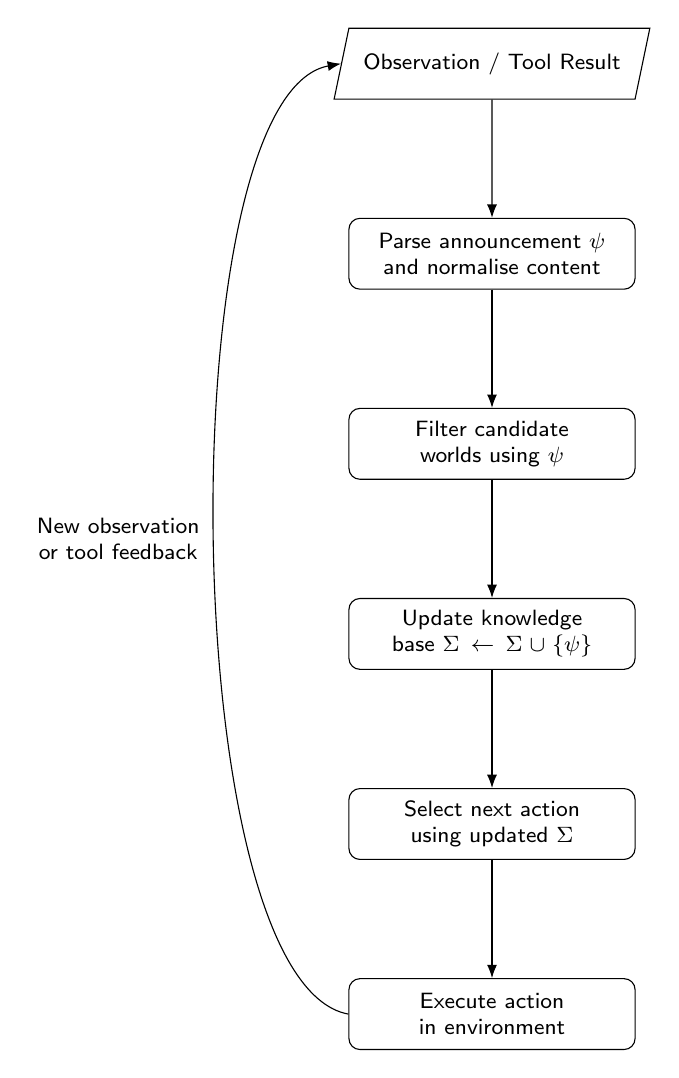
\begin{tikzpicture}[
      >=Latex,
      node distance=1.5cm,
      process/.style={draw, rounded corners, minimum height=0.9cm, text width=3.4cm, align=center, font=\footnotesize\sffamily},
      io/.style={draw, trapezium, trapezium stretches=true, trapezium left angle=70, trapezium right angle=110, minimum height=0.9cm, text width=3.4cm, align=center, font=\footnotesize\sffamily}
    ]
    \node[io] (observe) {Observation / Tool Result};
    \node[process, below=of observe] (parse) {Parse announcement $\psi$ and normalise content};
    \node[process, below=of parse] (filter) {Filter candidate worlds using $\psi$};
    \node[process, below=of filter] (log) {Update knowledge base $\Sigma \leftarrow \Sigma \cup \{\psi\}$};
    \node[process, below=of log] (decide) {Select next action using updated $\Sigma$};
    \node[process, below=of decide] (act) {Execute action in environment};

    \draw[->] (observe) -- (parse);
    \draw[->] (parse) -- (filter);
    \draw[->] (filter) -- (log);
    \draw[->] (log) -- (decide);
    \draw[->] (decide) -- (act);
    \draw[->] (act.west) .. controls +(-2.2,0.4) and +(-2.2,-0.4) .. node[left=2pt, align=center, font=\footnotesize\sffamily]{New observation\\or tool feedback} (observe.west);
  \end{tikzpicture}
  \caption{Epistemic update loop. Each observation is parsed into an announcement $\psi$, incorporated into the knowledge base $\Sigma$, and used to drive the agent's next action.}
  \label{fig:knowledge-flow}
\end{figure}


The cycle repeats while the agent interacts with the environment; query actions simply feed another announcement into the update stage until the task completes. Notably, this is similar to a POMDP belief update loop or a filtering loop in state estimation, as noted earlier. In those domains, after each sensor reading, the belief (a probability distribution or set of possible states) is updated. Here, $\Sigma$ is like a symbolic belief state being updated.

One might question: does this approach handle all kinds of knowledge an LLM might need? LLMs have a vast implicit world knowledge (from pre-training) that we are not explicitly enumerating in $\Sigma$. That's fine because $\Sigma$ is not meant to encode everything the model knows about the world, just the specific situation-specific knowledge. The model's background knowledge (like ``Paris is the capital of France'') is assumed to be available in its parameters. We only track things that are contingent on the current instance or that result from the current interaction. If needed, an LLM can always draw on its background knowledge; if it's important to the task, we may even represent a piece of it in $\Sigma$ for clarity (e.g., if the task is about geography, we might populate $\Sigma$ initially with relevant geographic facts retrieved from a knowledge base).

\subsection{Example: Tool-using LLM Agent with Epistemic Updates}
To ground the framework, let's walk through a more detailed scenario with a large language model agent that has to solve a problem by interacting with tools, and see how the epistemic state evolves. We'll include how the agent's prompts might look and how the system ensures consistency.

Scenario: The agent is an LLM assistant helping a user troubleshoot a network issue. The user says their internet is not working. The agent can use tools like ping\_test(host) which returns reachable or not, and dns\_lookup(domain) which returns an IP or failure.

Step 0: Initial knowledge $\Sigma_0$ might contain some generic assumptions or not. Let's say $\Sigma_0 = {}$ for simplicity.

Step 1 (User input): ``My internet is down. I cannot reach example.com.'' The agent parses this. It might interpret that as information: user cannot reach example.com. It could translate that to a fact like $\neg \text{Reachable}_{\text{user}}(\text{example.com})$. Suppose the agent does that. So it treats this as an announcement $\psi_1$: ``example.com not reachable from user's computer.'' Update: $\Sigma_1 = {
\neg \text{Reachable}_{\text{user}}(\text{example.com})}$.

Step 2 (Agent reasoning): The agent wants to diagnose. Possible issues: DNS problem or connectivity problem. It doesn't know the cause. It decides to use a tool: ping\_test(example.com). The tool returns: ``ping successful'' or perhaps ``host not found.'' Let's say the tool returns: ``ping: host not found.'' That is an announcement $\psi_2$: ``example.com DNS resolution failed.'' Now, this is new information. Update $\Sigma_2 = {
\neg \text{Reachable}_{\text{user}}(\text{example.com}), \; \text{DNSFail}(\text{example.com})}$.

From this, the agent might deduce: if DNS failed, it suggests a DNS issue. It knows (from its general knowledge, not explicitly in $\Sigma$ but background) that if DNS is failing, internet might actually be up but name resolution is the issue. So it now plans actions accordingly (maybe instruct user to check DNS settings). But to be sure, it could try another site by IP. However, let's say it deduces: internet is working but DNS is faulty. It might assert internally $\psi_3$: ``Connection is okay, DNS is the likely cause.'' We could formalize that if needed, but likely the agent just communicates it.

Step 3 (Agent output to user): ``It looks like a DNS issue. The domain name isn't resolving. Try changing your DNS server.'' Here it uses the knowledge it acquired.

The knowledge log at the end: $\Sigma = {
\neg \text{Reachable}_{\text{user}}(\text{example.com}), \text{DNSFail}(\text{example.com})}$. If later the user says ``Actually, I can reach sites by IP but not by name,'' that's consistent with the agent's knowledge (further confirming DNS problem, which was already the hypothesis).

Now, throughout this, the system could ensure the agent doesn't contradict itself. For example, the agent wouldn't say ``Maybe your internet cable is unplugged'' if it already concluded the ping reached the host (in our scenario ping didn't reach due to host not found, but a different scenario could yield contradictory leads).

This example shows how tool results feed epistemic updates. Each tool's answer is effectively a sensor reading that the agent adds to its knowledge state. In classical programming, one would just store it in a variable. The difference here is that by storing in $\Sigma$ and designing the logic around it, we can use logical inference (like eliminating possibilities, or triggering certain actions when something is known or unknown).

Listing~\ref{lst:diagnose-loop} demonstrates a small Python driver that applies the knowledge base to the connectivity scenario.

\lstinputlisting[language=Python, caption={Toy diagnostic loop that turns tool feedback into announcements.}, label={lst:diagnose-loop}]{code/pipeline_loop.py}

% Auto-generated from DOCX
\section{Implementation Considerations}
The theoretical framework is only useful if it can be implemented efficiently on top of LLMs. In this section, we discuss key practical considerations: ensuring the approach scales to the enormous proposition space of LLMs, dealing with partial observability and uncertainty, and integrating with the LLM's operation without requiring an entire logical reasoner that negates the advantages of the LLM.

\subsection{Scalability and Avoiding State Explosion}
One might fear that formalizing knowledge for an LLM (which can talk about virtually anything) would lead to an intractable state representation. After all, the set of possible ``worlds'' for an LLM that can generate arbitrary text is astronomically large. However, our approach is deliberately sparse. We never attempt to represent all those worlds; we only track the narrowing filter of what's been learned.

In practice, how many facts might an agent accumulate during a task? Possibly on the order of tens to low hundreds, even for complex tasks, because the agent will focus on task-relevant information. This is manageable. Each fact is likely a short sentence or predicate. Storing and checking a few hundred facts is trivial for a modern computer and can be kept within the LLM's context window if needed (especially as LLM context lengths grow). Moreover, if the number of facts grows too large, techniques like summarization can compress them. For example, if the agent has acquired a list of 20 clues in a murder mystery game, at some point it might synthesize them into higher-level theories and drop the minutiae.

Another angle to scalability is limiting reasoning depth. Full epistemic logic allows infinite chains like knowing that you know that you know... In our framework, we rarely need to go beyond one level (the agent knows X). We are not modeling another agent's mind in detail, so we don't have recursive knowledge except trivial common knowledge of the agent with itself. This dramatically simplifies things versus a general multi-agent epistemic model. We do not need to build huge Kripke structures; we just maintain a set of ground facts.

When it comes to inference, we also take a frugal approach. We are not employing an automated theorem prover to deduce all consequences of $\Sigma$. Instead, we rely on either simple direct checks or the LLM's own reasoning in most cases. For instance, to see if $\Sigma$ entails a certain condition, we could just prompt the LLM by providing $\Sigma$ and asking ``Given these facts, is it true that ...?'' The LLM is quite capable at basic logical reasoning when facts are explicitly given (and if it makes an error, we can double-check with a symbolic solver for safety on critical points).

Where needed, we can incorporate specific solvers for certain implications. For example, if some facts are numeric constraints, a linear solver could be used. But generally, since $\Sigma$ is small, even brute-force checking of combinations or using an SMT solver on it is feasible.

To connect with dynamic epistemic logic literature, Top et al. (2024) introduced the idea of bounded models in epistemic reasoning to deal with human subjects' limited reasoning depths\cite{pal-predictive}. Similarly, our agent is bounded: it will not consider arbitrarily complex hidden ramifications, only what it explicitly has logged or what it can derive with a few steps. In many cases, that's enough for practical performance, and it avoids the state space explosion of hypothetically considering everything.

\subsection{Partial Observability and Uncertainty}
Our framework inherently addresses partial observability: any fact not in $\Sigma$ is by default unknown to the agent. The agent may suspect or have probabilistic beliefs about unknowns, but until an announcement provides clarity, those possibilities remain open. In planning terms, the agent's belief state (the set of possible worlds consistent with $\Sigma$) often still contains multiple possibilities due to unknown factors. The agent can either act in a way that is safe despite the uncertainty (conformant planning) or perform sensing actions to reduce the uncertainty (conditional planning)\cite{pal-survey}.

One design is to explicitly mark certain propositions as unknown variables of interest, especially if we know the agent should resolve them. For example, if the task is to identify who among Alice or Bob has a secret, we could introduce a variable and note $\Sigma$ contains ``SecretHolder $\in \{Alice, Bob\}$'' initially. Then as evidence comes, that set narrows. This is akin to how programmers might maintain a list of suspects in code. In an LLM, one could simply ask the model to list possible candidates and update that list. Our approach gives a bit more rigor: the model can maintain in $\Sigma$ a disjunction or a set enumerating possibilities.

In terms of uncertainty, as discussed earlier, one could enrich $\Sigma$ with notations for belief degrees. For an initial implementation, one might not do full fuzzy logic but a simpler scheme: tag facts with confidence levels. E.g. ``(0.9) It is likely raining.'' If a conflicting fact comes, you might downgrade or replace. Some recent LLM self-evaluation techniques have the model assign likelihood scores to its statements. Those could feed into such tags. While we won't implement a full uncertain reasoning system here, it's good to note that nothing in the framework prevents storing ``probably X'' as a record. The query function then must interpret what to do if something is only probable.

If the environment can lie or be noisy, the agent could adopt a cautious approach: treat announcements as beliefs, not guaranteed truth, unless verified. For instance, if a tool is unreliable, the agent might add ``Tool said Y'' to $\Sigma$ rather than ``Y'', and keep a separate rule ``usually Tool is correct'' or a probability. Then it could cross-check via another tool or logic. This complicates things, but it shows the flexibility: $\Sigma$ can store not just direct facts but also source attributions or modal statements like $B (\text{Y})$ meaning ``the agent (just) believes Y tentatively''. A full dynamic doxastic logic (belief change) would allow modeling how beliefs get strengthened or weakened with evidence\cite{del-sep}. For now, in demonstration, we assume our sources are correct, so knowledge is monotonic.

One interesting challenge is knowledge forgetting or time. In a long-lived agent, facts in $\Sigma$ might become outdated (like step 5 in Table 1, where treasure moved, the old fact became invalid). One way to incorporate time is to timestamp facts or partition $\Sigma$ by context (like a world state that changes). A moving world is like a new scenario; announcements can be tagged as ``as of time t, $\phi$ is true''. Then if at time t+1 something changes, one can update accordingly. In some dynamic epistemic logics, there are action models for things like factual changes (which aren't announcements, but actual world changes that agents then observe). Our framework can tie into that by if the environment is known to change, the agent's planning should account for needing to re-check facts after certain actions. But this goes into planning strategy more than the epistemic record-keeping. Perhaps a simpler approach: when facts might have changed, the agent can remove them or mark them stale and re-investigate. This is similar to cache invalidation in software.

\subsection{Integration with LLM Workflows}
How do we implement this in an LLM agent pipeline? A concrete architecture can be sketched as follows:
\begin{enumerate}[leftmargin=*]
  \item Maintain a persistent \texttt{KnowledgeBase} object that stores $\Sigma$ across turns.
  \item For each reasoning cycle:
  \begin{enumerate}[label=\alph*.]
    \item Prepend a concise summary of $\Sigma$ to the LLM prompt or inject it via a system message.
    \item Instruct the model to respect the known facts (e.g. ``You know the following facts... Do not contradict them'').
    \item Let the LLM produce an action or answer; execute tool calls as needed and capture structured results.
    \item Normalise results into announcements and call \texttt{KnowledgeBase.update}.
    \item Optionally scan the model's own statements for confident self-announcements to append to $\Sigma$.
  \end{enumerate}
\end{enumerate}

Listing~\ref{lst:knowledge-base} shows a minimal Python helper that realises this loop.

\lstinputlisting[language=Python, caption={Knowledge base helper for epistemic announcements.}, label={lst:knowledge-base}]{code/knowledge_base.py}

The KnowledgeBase.update(info) needs some logic to interpret raw information into logical form. In some cases, it's straightforward (the tool returns structured data or a message we can map to a proposition). In others, if the LLM output says something like ``It might be A or B, not sure,'' we might encode that as uncertainty rather than a firm fact.

Using current tool-using agent frameworks (such as those built on top of LangChain or OpenAI functions), this integration is feasible: after each tool call, they often already inject the result into context. We'd additionally store it in a structured way.

Memory vs. KnowledgeBase: One might ask: the LLM has a context window and a kind of ``working memory'' in the prompt already; why not just rely on that for remembering things? The answer is twofold: (a) The context window is limited and might drop older info, whereas a separate knowledge store can persist arbitrarily. (b) More importantly, the knowledge base can be queried and manipulated symbolically. We can directly ask ``Does $\Sigma$ entail P?'' algorithmically, rather than relying on the LLM's sometimes unreliable recall. It's a form of verification and control. It also allows injecting absolute constraints (like if $\Sigma$ says ``Not X,'' we can forbid the model from outputting X as a solution, possibly by adding a high-weight penalty or an auxiliary classifier).

Interfacing with External Knowledge: If needed, the knowledge base could interface with external databases for domain knowledge. For example, if the agent needs to know capital cities, it might query Wiki and add ``Paris is capital of France'' to $\Sigma$. But one doesn't want to dump all Wikipedia; just relevant bits. This again highlights focusing on minimal relevant facts.

Epistemic Queries in Prompts: We can even have the LLM reason about its knowledge by asking it directly. For instance, ``Given the above facts, is it possible that ...?'' The LLM might say ``No, because fact X rules that out.'' This is a way to double-check its understanding. If it answered incorrectly, the system could intervene (maybe using a formal check or a second chain-of-thought) to correct it.

\subsection{Limits of Introspection and Resource Bounds}
While our framework gives structure, it doesn't magically make the LLM perfect. The model might still fail to use the knowledge correctly, especially under resource limitations or if the prompt becomes too long. We must ensure the prompt formatting is efficient and that the model is guided not to ignore $\Sigma$. Empirically, one might need to experiment with prompt styles (bullet lists of facts, or a brief narrative summary of known state) to see what the model best utilizes.

Another limitation is that the LLM might not always realize a needed knowledge gap without explicit training. By implementing these checks (like not proceeding if something isn't known), we sometimes override the model's own tendency. This is desirable for safety/consistency, but we should also allow the model's flexibility. The key is to strike a balance: enforce what's absolutely logically required, but let the model's creativity fill the rest. For instance, we wouldn't restrict the model's ability to generate hypotheses beyond $\Sigma$ (it can imagine things), but we would restrict it from stating those hypotheses as known facts unless they're deduced or verified.

Scalability not only refers to number of facts, but to the complexity of tasks (multi-step reasoning etc.). If tasks become extremely complex, the knowledge log might become large, but as argued, summarization or hierarchical reasoning can mitigate that. The agent could break a task into sub-tasks, each with its own sub-$\Sigma$ that gets merged or summarized into higher-level $\Sigma$.

Open-World vs Closed-World: Our approach implicitly assumes a kind of open-world scenario: not knowing $\varphi$ doesn't mean $\neg \varphi$ is assumed. The agent doesn't fill unknowns with defaults unless told. This is usually correct for real-world tasks. But sometimes a closed-world assumption is used (if something is not known true, assume false). We have to be careful: For example, if $\Sigma$ doesn't have ``key is present'', the agent shouldn't automatically assume ``key is not present''; it should recognize it as unknown and either ask or search for it. So by default we treat unknown as unknown. If needed, a particular domain can impose closed-world (like in a puzzle where anything not stated is false, but that's rarely the case in open environments).

Finally, we consider how this could be evaluated, as that guides some implementation choices. If we create an agent with this framework, we should test it on scenarios requiring consistent knowledge updates. Reflection-Bench tasks\cite{reflection-bench}, for example, include dimensions like belief updating and memory. We would expect our agent to outperform a baseline LLM agent on tasks where tracking what is known is crucial (like solving a mystery without contradicting clues, or doing a treasure hunt where you must remember which locations were searched). An evaluation might measure success rate, number of mistakes like redundant questions or contradictions, etc. We discuss more on this in the next section.


% Auto-generated from DOCX
\section{Discussion}
The proposed framework brings together ideas from logic and the practical demands of LLM agent systems. Here, we reflect on the implications, compare with other approaches, and highlight challenges and future directions.

\subsection{Comparison with Related Approaches}
Classical AI Planning and BDI: Our method has echoes of classical knowledge-based planning and the BDI model. In knowledge-based planning, one explicitly represents the agent's beliefs and plans sensing actions to reduce uncertainty\cite{dynamic-term-modal}. Those approaches often required specialized planners or model checkers due to the complexity of epistemic reasoning. In contrast, we leverage the LLM's flexibility and only maintain a lightweight state. BDI architectures represent beliefs as a database, which is very similar to our $\Sigma$. The difference is that BDI usually doesn't formalize how the belief base is updated by perception in logical terms, and it's more an architectural concept. We add the PAL semantic flavor to it, making it clear that perceptions act like announcements that prune the belief base. Another difference: BDI often allows inconsistent beliefs (the agent can have beliefs that are wrong, until corrected), whereas we try to keep $\Sigma$ factually consistent with the environment (if our announcements are truthful).

Neuro-Symbolic and Knowledge Graph Augmented LLMs: There's a growing trend to combine neural and symbolic reasoning. One example is LLMs using a knowledge graph to get factual information and even to do logic queries. In our framework, the knowledge log $\Sigma$ could be seen as a tiny, dynamically built knowledge graph (just a set of triples or propositions). The difference from static knowledge graphs is that $\Sigma$ is highly context-specific and is built on the fly, rather than querying a huge static graph of world knowledge. Projects like KGA2 (Knowledge Graph-Augmented Agents) often focus on retrieving from a fixed knowledge base like Wikipedia, whereas we focus on logically updating a working knowledge set that pertains to the current problem.

Chain-of-Thought and Self-Reflection: LLMs with chain-of-thought (CoT) prompting do have some capacity to simulate belief updates by enumerating what they deduce step by step. Techniques like Scratchpad let the model write down intermediate results. One could argue that if an LLM were sufficiently advanced, it could internally simulate our entire framework without explicit structure. Possibly true, but current models show flaws in long or complex reasoning unless guided. By imposing structure, we reduce the cognitive load on the model, so it doesn't have to juggle all facts in pure text; we assist it by keeping a structured memory. Moreover, our approach is more transparent. It provides a trace (the $\Sigma$ log) that can be inspected or audited by humans or debugging tools. This is important for aligning AI behavior: one can see exactly ``why'' the agent thinks X (because fact Y is in $\Sigma$).

Approaches like Reflexion by Shinn et al. involve the model generating critiques of its answers and improving over iterations. That is orthogonal but complementary. One could incorporate a reflection step where after completing a task (or at certain milestones) the agent reviews $\Sigma$ for any contradictions or missed opportunities (like ``I still don't know X, should have asked that.''). The framework provides a scaffold for such meta reasoning, because $\Sigma$ is a concise summary of knowledge, it's easier to review than raw dialogue.

Memory Networks and Long Conversation Handling: Some research addresses long-term consistency by fine-tuning models to refer back to earlier conversation or use a separate memory module. Those often remain neural (vector-based retrieval). Our approach could easily incorporate vector search to fetch relevant past facts into $\Sigma$ if the agent has a long history. For instance, if the agent handled a user's device setup last month, and now the user returns with an issue, a memory system might surface ``User has model X router, set up last month.'' That can be put into $\Sigma$ as prior knowledge. So, this doesn't replace vector memory; it works with it. The key is the retrieved memory is then treated logically: if it says ``the router password is ABC'', then $\Sigma$ will ensure the agent doesn't act as if it's unknown.

\subsection{Benefits and Limitations}
\paragraph{Benefits.}
\begin{itemize}
  \item \textbf{Consistency.} An explicit record drastically reduces contradictory or repetitive actions, a common failure mode for LLM agents.
  \item \textbf{Interpretability.} The knowledge log exposes the provenance of each conclusion, easing debugging and human oversight.
  \item \textbf{Goal-driven information gathering.} By recognising unknowns, the agent proactively seeks announcements to close gaps, improving task efficiency\cite{reflection-bench}.
  \item \textbf{Modularity.} The epistemic layer wraps around the LLM and can be paired with different backends or deployment contexts without major changes.
\end{itemize}

\paragraph{Limitations.}
\begin{itemize}
  \item \textbf{Bootstrapping assumptions.} Incorrect initial facts can persist in $\Sigma$ until explicitly revised, so the agent needs mechanisms for correction.
  \item \textbf{Incomplete reasoning.} Without full logical closure, simple entailments might be missed unless assisted by lightweight inference add-ons.
  \item \textbf{Operational overhead.} Managing the prompt and knowledge base adds cost, though it is justified on tasks that demand consistency.
  \item \textbf{Model compliance.} The LLM must respect authoritative facts; guard rails such as post-generation checks help when hallucinations occur.
  \item \textbf{Multi-agent complexity.} Extending the framework to shared or divergent knowledge states across agents requires additional bookkeeping beyond the current scope.
\end{itemize}

\subsection{Open Challenges}
Several open research questions arise from this work:
\begin{enumerate}[leftmargin=*]
  \item \textbf{Learning structured knowledge outputs.} Can models be trained to emit machine-readable KNOW statements, reducing the need for bespoke parsers?
  \item \textbf{Robustness to misinformation.} What belief-revision strategies help resolve conflicts between trusted sources, and how can LLMs assist in diagnosing the culprit\cite{del-sep}?
  \item \textbf{Resource-aware prompting.} How do we keep prompts compact, perhaps by querying $\Sigma$ on demand or caching filtered summaries instead of replaying the full log each turn?
  \item \textbf{Evaluation metrics.} Purpose-built benchmarks (e.g. Reflection-Bench\cite{reflection-bench}) should measure contradictions avoided, redundant actions, or success rates on epistemic puzzles.
  \item \textbf{Human-agent common ground.} Extending the framework to reason about the user's knowledge could support richer dialogue strategies and aligns with prior discourse modelling. %Need citation

\end{enumerate}

\subsection{Toward Structured Cognition in LLMs}
One way to view our framework is as a step towards structured cognition or a form of System II reasoning layered on top of the LLM's System I fluency. The LLM provides the intuition, language fluency, and associative knowledge; the logic layer provides structuring, memory, and consistency. This combination is reminiscent of dual-process theory in cognitive science, where logical reasoning can override automatic impulses when needed.

We believe this kind of architecture will become increasingly important as LLM agents tackle more complex, multi-step problems. The alternative is to try to train end-to-end LLMs to handle everything internally, but that may require orders of magnitude more parameters or data, and even then interpretability would suffer. By explicitly structuring part of the problem (state management), we guide the model and reduce the search space it has to navigate.

This framework is also model-agnostic: it could work with GPT-4, or an open-source Llama, etc. If an LLM improves in reliability, the logic layer doesn't hinder it; it only steps in to enforce consistency. In fact, a stronger LLM might make even better use of $\Sigma$, drawing more subtle inferences. A weaker LLM might need more explicit inference rules coded (like we might have to manually implement transitivity or other reasoning it fails at).

Generality: While our examples have been in text-based domains, the concept applies to any agent that uses an LLM for planning or decision. For instance, a robot with an LLM-based planner could maintain a knowledge state about its environment (objects seen, locations clear, etc.). The announcements are then sensor readings or map updates, and $\Sigma$ ensures it doesn't, say, attempt to walk through a region it knows is blocked. Traditional robotics already has SLAM (simultaneous localization and mapping), which is essentially building a knowledge state (a map). Our contribution is more relevant in abstract or informational environments where the ``map'' is not spatial but logical (like puzzle states, dialogue facts, etc.).

\subsection{Future Work}
Advanced Logic Integration: We can consider integrating more advanced dynamic epistemic logic constructs like action models. Public announcements are one type of epistemic action, but there are others like private announcements (where only one agent hears something), or deceptive announcements. In multi-agent systems, one could model communication by one agent as an announcement that updates others but not the sender's own knowledge (or the sender already knew it). Implementing such things might be needed for, say, two LLM agents cooperating or negotiating.

Automated Knowledge Extraction: Using LLMs themselves to extract facts from unstructured content (like long documents) into $\Sigma$ would be useful. Many LLM agents already do some form of summarization or extraction when using tools (e.g., browsing a webpage and noting key points). If we align that with our epistemic approach, the agent could explicitly say, ``From the document, I learned: Fact1, Fact2.'' Those go into $\Sigma$. If done well, this could vastly improve the agent's ability to handle long inputs by distilling them into a knowledge base it can reason with, instead of juggling long text in context.

Dynamic Prioritization: Not all facts in $\Sigma$ are equally important at all times. Perhaps a mechanism to mark some as core vs peripheral would help. If the context window is limited, maybe only feed core ones unless needed. This is similar to how humans keep salient facts in mind and others in the background.

Incorporating Learning: Over repeated tasks, the agent could learn which epistemic strategies work best. Perhaps it might refine a policy like ``always clarify unknown goal parameters early.'' Our framework makes such strategies more viable because the agent can detect unknowns easily. An interesting direction is letting the agent simulate possible outcomes based on current $\Sigma$. It could imagine, ``If I continue with this plan and my unknown X turns out to be true, what then? If false, what then?'' This is essentially contingent planning. The logic layer could spawn hypothetical branches for each case of X, and the LLM could plan in each branch. While computationally heavy, for small numbers of key unknowns it might be doable. This would lead to very robust decision-making (covering all cases), but guiding an LLM to do that systematically is a research challenge.

In conclusion, our approach is a step toward marrying the strengths of LLMs (flexible reasoning, knowledge, language use) with the rigor of logical state tracking. It provides a blueprint for building AI agents that can know what they know (and don't know) in a principled way. This not only improves performance on many tasks but is also essential for safety, because an agent that is aware of its knowledge limits can avoid overconfidently giving wrong answers or taking dangerous actions.


% Auto-generated from DOCX
\section{Conclusion}
We have presented a framework for applying public announcement logic (PAL) and related epistemic logic principles to manage the knowledge state of LLM-based agents. By representing the agent's knowledge as a minimal set of facts (announcements) and updating this set whenever new information is obtained, the agent effectively simulates the elimination of possible worlds without ever enumerating them. This approach brings several advantages: the agent maintains consistency, can explicitly reason about what it knows or doesn't know, and can plan information-gathering actions accordingly. We grounded key epistemic concepts, including possible worlds, knowledge modalities, common knowledge, and announcements, in the context of LLM agent workflows, illustrating with examples how an agent's log of observations serves as an epistemic filter on its beliefs\cite{espf}. We also discussed extensions to graded and fuzzy modal logics, acknowledging that real-world agents operate under uncertainty and may assign degrees of belief rather than certainties\cite{del-sep}. While our current implementation treats incoming information as truthful knowledge updates (public announcements in the strict sense\cite{del-sep}), the framework is flexible enough to accommodate belief updates with less than full certainty, using plausibility or probability-based reasoning from dynamic doxastic logic\cite{del-sep}.

Our framework essentially functions as a protocol layer for structured cognition in LLM agents, independent of the underlying language model. It interfaces with the LLM by feeding it the up-to-date knowledge state and intercepting its outputs for new potential facts. This creates a positive feedback loop: as the LLM derives or discovers information, the state is updated, which in turn informs subsequent reasoning. We showed that this approach can be integrated into existing agent architectures that use chain-of-thought prompting and tool use, with relatively low overhead. The payoff is that the agent avoids many pitfalls such as forgetting earlier information, contradicting itself, or blindly guessing in the face of unknowns. Especially as tasks become long or collaborative, having an explicit notion of ``what we (agent or team) know so far'' becomes crucial. Our approach offers an implementable solution to that, inspired by decades of research in epistemic logic and multi-agent systems.

There are, of course, challenges and open questions remaining. We need to further develop methods for belief revision when the agent encounters contradictions, possibly leveraging the LLM's reasoning to decide which prior assumptions to drop. We also should explore how the framework scales in truly open-ended environments, where new propositions can continuously appear. The worry of unbounded proposition space is mitigated by the agent's focus on relevant info, but formal assurances (e.g. complexity analysis, or constraints on $\Sigma$ growth) would strengthen the approach. On the evaluation front, we propose constructing benchmarks that specifically test an agent's ability to update and use its knowledge state, such as puzzle-solving tasks, or simulated exploration tasks where remembering visited locations matters. By comparing an agent with and without our epistemic layer, we can quantify improvements in correctness and efficiency (e.g., fewer redundant actions, higher success rate on tasks requiring memory of past clues).

In terms of impact and applicability, this framework could enhance any AI system that requires a mix of learning and reasoning. A few examples include: virtual assistants that must keep track of user preferences across sessions, autonomous scientific discovery systems that accumulate findings and must avoid contradicting prior evidence, and multi-agent teams (human-AI or AI-AI) where maintaining a shared knowledge base is key to coordination. By formalizing the knowledge updates, we provide a clear interface for trust: a human supervisor could inspect the knowledge log $\Sigma$ to verify if the agent is operating on correct information. This is an advantage over end-to-end neural methods where the internal state is a opaque vector.

Finally, we note that our work sits at an intersection of symbolic and neural methods, and exemplifies how insights from logic can help tackle modern AI problems. The use of PAL, a relatively niche logical framework, in a cutting-edge LLM scenario is a testament to the enduring relevance of symbolic reasoning for AI's explainability and reliability. As LLMs become more capable, ensuring they have robust internal states and know when to seek information will be increasingly important. We believe the ideas presented here are a step toward LLM agents that are not just linguistically competent, but epistemically self-aware.





\bibliographystyle{unsrt}
\bibliography{references}

\end{document}
